\documentclass[10pt,a4paper]{article}
\usepackage[margin=0.62in]{geometry}
\usepackage[T1]{fontenc}
\usepackage[utf8]{inputenc}
\usepackage{lmodern}
\usepackage{amsmath,amssymb}
\usepackage{booktabs}
\usepackage{tabularx}
\usepackage{array}
\usepackage{graphicx}
\usepackage{float}
\usepackage{subcaption}
\usepackage{enumitem}
\usepackage{xcolor}
\usepackage{hyperref}
\usepackage{microtype}
\usepackage{titlesec}
\usepackage{fancyhdr}
\usepackage[most]{tcolorbox}
\usepackage{tikz}
\usetikzlibrary{positioning,arrows.meta,calc,shapes.geometric,decorations.pathreplacing}

\definecolor{brand}{HTML}{0D3B66}
\definecolor{accent}{HTML}{2A9D8F}
\definecolor{softbg}{HTML}{F4F8FB}
\definecolor{textdark}{HTML}{1E1E1E}

\hypersetup{
  colorlinks=true,
  linkcolor=brand,
  urlcolor=accent
}

\setlength{\parindent}{0pt}
\setlength{\parskip}{3pt}
\setlist[itemize]{leftmargin=1.2em,itemsep=1pt,topsep=2pt}

\titleformat{\section}{\color{brand}\large\bfseries}{\thesection.}{0.4em}{}
\titleformat{\subsection}{\color{textdark}\bfseries}{\thesubsection}{0.4em}{}
\titlespacing*{\section}{0pt}{8pt}{4pt}
\titlespacing*{\subsection}{0pt}{6pt}{3pt}

\pagestyle{fancy}
\fancyhf{}
\fancyhead[L]{\small CS671 Technical Model Report}
\fancyhead[R]{\small CycleGAN (Pelvis)}
\fancyfoot[C]{\small \thepage}
\setlength{\headheight}{14pt}

\begin{document}

% -------------------- Header Block --------------------
\begin{tcolorbox}[
  enhanced,
  colback=softbg,
  colframe=brand,
  boxrule=0.9pt,
  arc=2mm,
  left=5pt,right=5pt,top=5pt,bottom=5pt
]
\centering
{\Large\bfseries\color{brand} CS671 -- Deep Learning and Its Applications}\\[2pt]
{\large\bfseries Technical Documentation Report}\\[6pt]
{\normalsize\bfseries Model: CycleGAN (Pelvis)}\\[4pt]
\small
Project Group: 5 \quad Region: Pelvis \quad Modality: Unpaired (CT $\leftrightarrow$ MRI)
\end{tcolorbox}

\section{ARCHITECTURAL OVERVIEW}
CycleGAN enables unpaired image-to-image translation by learning a mapping $G: X \to Y$ and $F: Y \to X$ such that the dynamics of the domains are preserved through cycle consistency. In this implementation for Pelvis CT-MRI translation, we utilize a ResNet-based generator and a PatchGAN discriminator to ensure high-fidelity anatomical preservation without requiring perfectly aligned training pairs.

\subsection{Generator Architecture (ResNet-9)}
The generator $G_{CT \to MRI}$ is implemented as a deep ResNet-9 architecture, specifically adapted for the $256 \times 256$ SynthRAD slices. This architecture utilizes a residual bottleneck to maintain structural integrity across the domain translation.

\begin{figure}[H]
\centering
\resizebox{\textwidth}{!}{
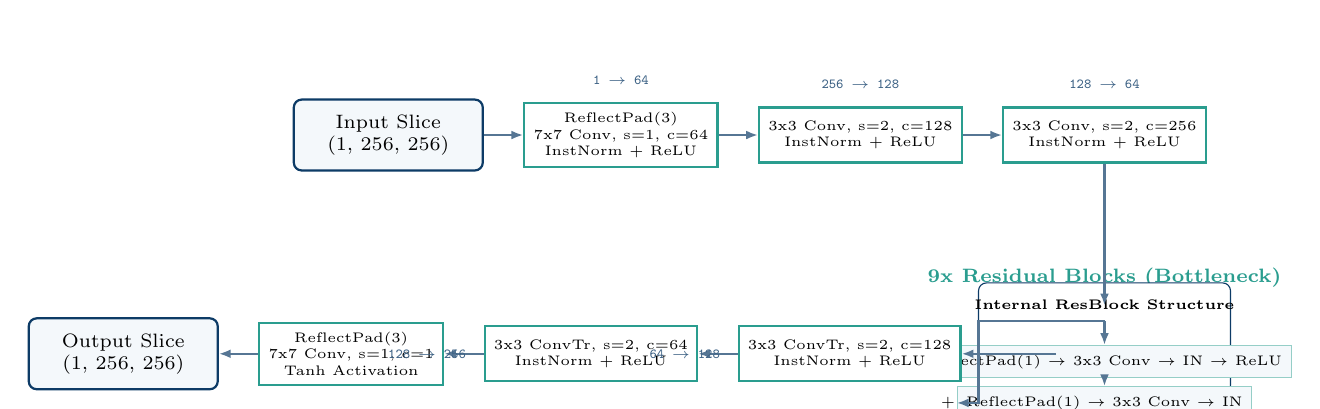
\begin{tikzpicture}[
    node distance=5mm,
    block/.style={draw=brand, thick, fill=softbg, minimum width=2.4cm, minimum height=0.9cm, align=center, rounded corners=1mm, font=\scriptsize},
    module/.style={draw=accent, thick, fill=white, minimum width=2.0cm, minimum height=0.7cm, align=center, font=\tiny},
    tensor/.style={font=\tiny\ttfamily, color=brand!80},
    arr/.style={-{Latex[length=1.5mm]}, thick, draw=brand!70}
]
    % Encoder path
    \node[block] (in) {Input Slice\\(1, 256, 256)};
    \node[module, right=of in] (c1) {ReflectPad(3)\\7x7 Conv, s=1, c=64\\InstNorm + ReLU};
    \node[module, right=of c1] (d1) {3x3 Conv, s=2, c=128\\InstNorm + ReLU};
    \node[module, right=of d1] (d2) {3x3 Conv, s=2, c=256\\InstNorm + ReLU};
    
    % Bottleneck
    \node[draw=accent, dashed, thick, fill=accent!5, rounded corners=2mm, inner sep=6mm, below=1.8cm of d2] (resnet_box) {};
    \node[font=\scriptsize\bfseries, color=accent, above=1mm of resnet_box] {9x Residual Blocks (Bottleneck)};
    
    % Detail of one ResBlock
    \begin{scope}[shift={(resnet_box.center)}, yshift=2mm]
        \node[draw=brand, fill=white, minimum width=3.2cm, minimum height=1.4cm, rounded corners=1mm] (inner_block) {};
        \node[font=\tiny\bfseries, below=1mm of inner_block.north] {Internal ResBlock Structure};
        \node[draw=accent!50, fill=softbg, minimum width=2.8cm, minimum height=0.4cm, font=\tiny, yshift=-3mm] (layer1) at (inner_block.center) {ReflectPad(1) $\to$ 3x3 Conv $\to$ IN $\to$ ReLU};
        \node[draw=accent!50, fill=softbg, minimum width=2.8cm, minimum height=0.4cm, font=\tiny, below=1mm of layer1] (layer2) {ReflectPad(1) $\to$ 3x3 Conv $\to$ IN};
        \draw[arr] (layer1) -- (layer2);
        \draw[arr] ($(layer1.north) + (0,0.3)$) -- (layer1.north);
        \draw[arr] ($(layer1.north) + (0,0.3)$) -- ++(-1.6,0) |- (layer2.west) node[pos=0.8, left, font=\tiny] {+};
    \end{scope}

    % Decoder path
    \node[module, left=1.2cm of resnet_box] (u1) {3x3 ConvTr, s=2, c=128\\InstNorm + ReLU};
    \node[module, left=of u1] (u2) {3x3 ConvTr, s=2, c=64\\InstNorm + ReLU};
    \node[module, left=of u2] (out_conv) {ReflectPad(3)\\7x7 Conv, s=1, c=1\\Tanh Activation};
    \node[block, left=of out_conv] (out) {Output Slice\\(1, 256, 256)};

    % Connections
    \draw[arr] (in) -- (c1);
    \draw[arr] (c1) -- (d1);
    \draw[arr] (d1) -- (d2);
    \draw[arr] (d2) -- (resnet_box.north);
    \draw[arr] (resnet_box.west) -- (u1);
    \draw[arr] (u1) -- (u2);
    \draw[arr] (u2) -- (out_conv);
    \draw[arr] (out_conv) -- (out);

    % Tensors flow labels
    \node[tensor, above=1mm of c1] {1 $\to$ 64};
    \node[tensor, above=1mm of d1] {256 $\to$ 128};
    \node[tensor, above=1mm of d2] {128 $\to$ 64};
    \node[tensor, left=1mm of u1] {64 $\to$ 128};
    \node[tensor, left=1mm of u2] {128 $\to$ 256};
\end{tikzpicture}
}
\caption{Detailed Generator Architecture: Utilizing Reflection Padding to maintain boundary continuity and Instance Normalization for robust cross-modal feature alignment.}
\end{figure}

\textbf{Tensor Flow and Feature Extraction:} 
The implementation follows a precise dimensionality transition: $(1, 256, 256) \xrightarrow{Encoder} (256, 64, 64) \xrightarrow{Bottleneck} (256, 64, 64) \xrightarrow{Decoder} (1, 256, 256)$. By compressing the spatial dimensions by a factor of 4 while expanding the channel depth to 256, the network extracts deep semantic features (e.g., pelvic bone structure and bladder boundaries) while the 9 residual blocks in the bottleneck allow the model to learn complex tissue mappings without losing global structural alignment.

\textbf{Anatomical Preservation via Residual Learning:} 
Each residual block implements the mapping $y = \text{ReLU}(f(x) + x)$. The use of \texttt{ReflectionPad2d} is critical in pelvic imaging to avoid boundary artifacts, ensuring that external contours and delicate internal organs like the prostate are translated without edge distortion.

\subsection{Discriminator Architecture (70x70 PatchGAN)}
The discriminator $D_{Y}$ uses a PatchGAN architecture to penalize local image patches, promoting the synthesis of high-frequency anatomical textures.

\begin{figure}[H]
\centering
\resizebox{0.9\textwidth}{!}{
\begin{tikzpicture}[
    node distance=6mm,
    block/.style={draw=brand, thick, fill=softbg, minimum width=2.4cm, minimum height=0.8cm, align=center, rounded corners=1mm, font=\scriptsize},
    module/.style={draw=brand!70, thick, fill=white, minimum width=2.0cm, minimum height=0.6cm, align=center, font=\tiny},
    arr/.style={-{Latex[length=1.5mm]}, thick, draw=accent}
]
    \node[block] (in) {Synthetic MRI\\(1, 256, 256)};
    \node[module, right=of in] (c1) {4x4 Conv, s=2, c=64\\LeakyReLU(0.2)};
    \node[module, right=of c1) (c2) {4x4 Conv, s=2, c=128\\InstNorm + LReLU};
    \node[module, right=of c2] (c3) {4x4 Conv, s=2, c=256\\InstNorm + LReLU};
    \node[module, right=of c3] (c4) {4x4 Conv, s=1, c=512\\InstNorm + LReLU};
    \node[module, right=of c4] (head) {4x4 Conv, s=1, c=1\\Patch Output};
    \node[block, below=8mm of head] (out) {30x30 Logit Grid\\(Real / Fake)};

    \draw[arr] (in) -- (c1);
    \draw[arr] (c1) -- (c2);
    \draw[arr] (c2) -- (c3);
    \draw[arr] (c3) -- (c4);
    \draw[arr] (c4) -- (head);
    \draw[arr] (head) -- (out);

    % Dimensionality labels
    \node[font=\tiny\ttfamily, color=brand!70, above=1mm of c1] {128x128};
    \node[font=\tiny\ttfamily, color=brand!70, above=1mm of c2] {64x64};
    \node[font=\tiny\ttfamily, color=brand!70, above=1mm of c3] {32x32};
    \node[font=\tiny\ttfamily, color=brand!70, above=1mm of head] {30x30};
\end{tikzpicture}
}
\caption{PatchGAN Discriminator: Hierarchical convolutions provide a $70 \times 70$ receptive field for local texture evaluation.}
\end{figure}

\textbf{Receptive Field and Local Consistency:} 
Instead of a single output scalar, the discriminator produces a $30 \times 30$ grid. This forces the generator to achieve realistic contrast in every local region, which is essential for distinguishing prostate tissue from surrounding muscle and fat layers in MRI.

\section{TRAINING DYNAMICS}
The model is trained using a composite loss function to ensure both realism and cycle consistency.

\begin{figure}[H]
\centering
\resizebox{0.85\textwidth}{!}{
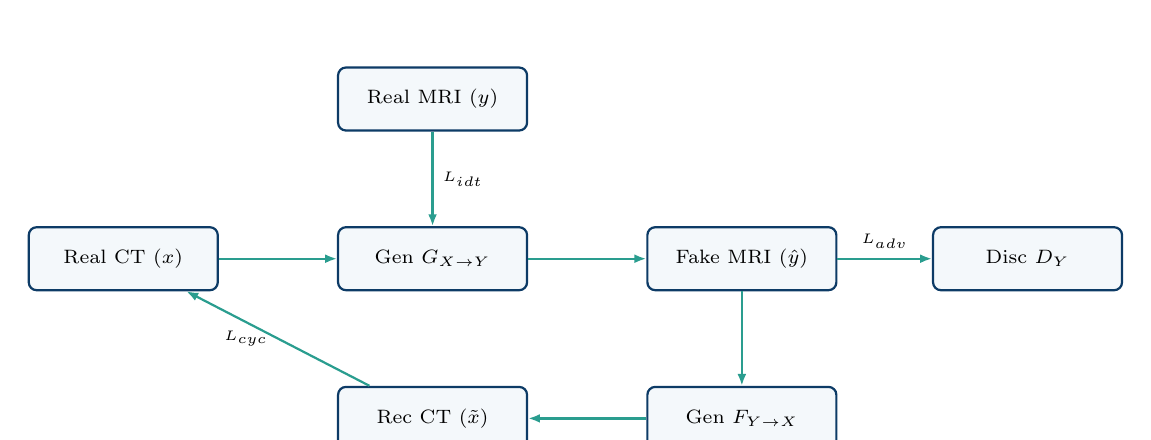
\begin{tikzpicture}[
    node distance=10mm,
    box/.style={draw=brand, thick, fill=softbg, minimum width=2.4cm, minimum height=0.8cm, align=center, rounded corners=1mm, font=\scriptsize},
    loss/.style={draw=accent, thick, fill=accent!5, minimum width=2.2cm, minimum height=0.7cm, align=center, font=\tiny\bfseries},
    arr/.style={-{Latex[length=1.5mm]}, thick, draw=accent}
]
    % Loop X -> Y -> X
    \node[box] (x) {Real CT ($x$)};
    \node[box, right=1.5cm of x] (gy) {Gen $G_{X \to Y}$};
    \node[box, right=1.5cm of gy] (fakey) {Fake MRI ($\hat{y}$)};
    \node[box, below=1.2cm of fakey] (fx) {Gen $F_{Y \to X}$};
    \node[box, left=1.5cm of fx] (recx) {Rec CT ($\tilde{x}$)};

    \draw[arr] (x) -- (gy);
    \draw[arr] (gy) -- (fakey);
    \draw[arr] (fakey) -- (fx);
    \draw[arr] (fx) -- (recx);
    \draw[arr] (recx) -- (x) node[midway, left, font=\tiny] {$L_{cyc}$};

    % Discriminator
    \node[box, right=1.2cm of fakey] (dy) {Disc $D_Y$};
    \draw[arr] (fakey) -- (dy) node[midway, above, font=\tiny] {$L_{adv}$};

    % Identity
    \node[box, above=1.2cm of gy] (realy) {Real MRI ($y$)};
    \draw[arr] (realy) -- (gy) node[midway, right, font=\tiny] {$L_{idt}$};
\end{tikzpicture}
}
\caption{Training Workflow: Interaction between Adversarial, Cycle, and Identity losses.}
\end{figure}

\textbf{Loss Objectives and Implementation Details:}
\begin{itemize}
    \item \textbf{Adversarial Loss ($L_{adv}$):} Implemented via \texttt{MSELoss} (LSGAN) to ensure stable training and avoid vanishing gradients.
    \item \textbf{Cycle Consistency Loss ($L_{cyc}$):} Enforces $F(G(x)) \approx x$ using $L_1$ loss, ensuring anatomical consistency.
    \item \textbf{Identity Loss ($L_{idt}$):} Prevents the generator from changing the color distribution when the target modality is provided as input.
    \item \textbf{Volume Conservation Loss ($L_{vol}$):} A custom regularizer penalizing local structure expansion/contraction via Jacobian determinant constraints.
    \item \textbf{Edge Loss ($L_{edge}$):} A gradient-difference loss targeted at preserving sharp organ boundaries in the pelvic region.
\end{itemize}

\section{INFERENCE PIPELINE}
The inference process translates 3D volumes by processing them as a sequence of independent 2D axial slices.

\begin{figure}[H]
\centering
\resizebox{0.9\textwidth}{!}{
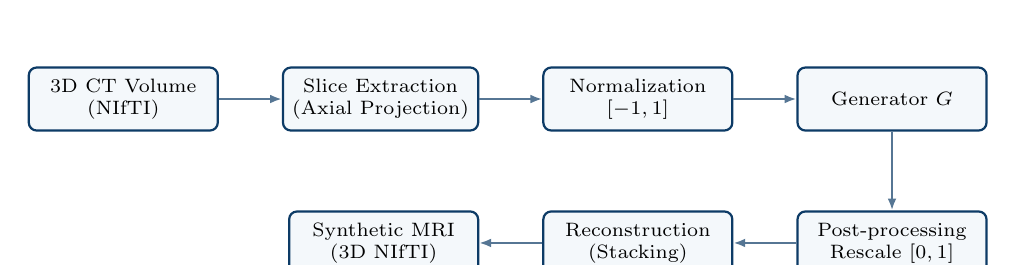
\begin{tikzpicture}[
    node distance=8mm,
    block/.style={draw=brand, thick, fill=softbg, minimum width=2.4cm, minimum height=0.8cm, align=center, rounded corners=1mm, font=\scriptsize},
    arr/.style={-{Latex[length=1.5mm]}, thick, draw=brand!70}
]
    \node[block] (v) {3D CT Volume\\(NIfTI)};
    \node[block, right=of v] (s) {Slice Extraction\\(Axial Projection)};
    \node[block, right=of s] (n) {Normalization\\$[-1, 1]$};
    \node[block, right=of n] (g) {Generator $G$};
    \node[block, below=1cm of g] (r) {Post-processing\\Rescale $[0, 1]$};
    \node[block, left=of r] (f) {Reconstruction\\(Stacking)};
    \node[block, left=of f] (out) {Synthetic MRI\\(3D NIfTI)};

    \draw[arr] (v) -- (s);
    \draw[arr] (s) -- (n);
    \draw[arr] (n) -- (g);
    \draw[arr] (g) -- (r);
    \draw[arr] (r) -- (f);
    \draw[arr] (f) -- (out);
\end{tikzpicture}
}
\caption{End-to-end inference workflow from volume ingestion to reconstruction.}
\end{figure}

The inference engine performs intensity normalization to match the training distribution. After the forward pass through the ResNet generator, the synthetic slices are re-stacked into a 3D tensor, ensuring that the affine transformation matrix from the original NIfTI header is preserved for clinical spatial alignment.

\end{document}
